\documentclass{standalone}

\usepackage{tikz}
\usepackage{circuitikz}
\usetikzlibrary{shapes,arrows}

\tikzset{>=stealth',every on chain/.append style={join},
         every join/.style={->}}

\tikzstyle{block} = [rectangle, draw, text centered, rounded corners, minimum
height=4cm, minimum width=0.5cm]

\tikzstyle{Mblock} = [rectangle, draw, text centered, rounded corners, minimum
height=0.5cm, minimum width=0.25cm]

\tikzstyle{blank} = [node distance = 0.8cm]
\tikzstyle{connectPoint} = [node distance = 1cm,circle,fill=black, inner sep= 0.5pt]

\tikzstyle{line} = [draw,->]
\tikzstyle{lineC} = [draw]

\tikzstyle{phaseShifter} = [circle,draw]


\begin{document}
 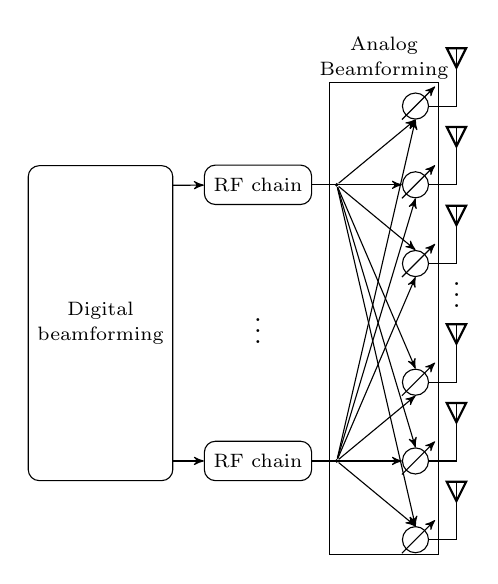
\begin{tikzpicture}

   \node[block] (dBeam) {\scriptsize{\shortstack{Digital \\ beamforming}}};

   \node[Mblock] (RF1) [right of = dBeam, right = 1.cm, above = 1.5cm] {\scriptsize{RF chain}};
   \node[Mblock] (RF2) [below of = RF1,below = 2.25cm] {\scriptsize{RF chain}};

   \node[blank]  (p1)  at (dBeam.east)[yshift=1.75 cm,xshift=-0.13cm] {};
   \node[blank]  (p2)  at (dBeam.east)[yshift=-1.75 cm,xshift=-0.13cm] {};

   \node[blank]  (dots) [below of = RF1, yshift = -0.95cm] {$\vdots$};

   \node[connectPoint]  (nodeInOut1) [right of = RF1] {};
   \node[connectPoint]  (nodeInOut2) [right of = RF2] {};


   % Phase shifters of RF chains One
   \node[phaseShifter] (P1) [right of = nodeInOut1] {} ;
   \node[phaseShifter] (P2) [above of = P1] {} ;
   \node[phaseShifter] (P3) [below of = P1] {} ;


   % Phase shifters of RF chains One
   \node[phaseShifter] (W1) [right of = nodeInOut2] {} ;
   \node[phaseShifter] (W2) [above of = W1] {} ;
   \node[phaseShifter] (W3) [below of = W1] {} ;

   %% Lines

   \path[line] (p1) -- (RF1);
   \path[line] (p2) -- (RF2);
   \path[line] (RF1) -- (P1);
   \path[line] (nodeInOut1) -- (P2.south);
   \path[line] (nodeInOut1) -- (P3.north);
   \path[line] (nodeInOut1) -- (W3.north);
   \path[line] (nodeInOut1) -- (W2.north);
   \path[line] (nodeInOut1) -- (W1.north);


   \path[line] (RF2) -- (W1);
   \path[line] (nodeInOut2) -- (W2.south);
   \path[line] (nodeInOut2) -- (W3.north);

   \path[line] (nodeInOut2) -- (P3.south);
   \path[line] (nodeInOut2) -- (P2.south);
   \path[line] (nodeInOut2) -- (P1.south);



 %% Antennas  

   \node[antenna,scale=0.35] (antP1) at (P1.east)[xshift=1cm] {};
   \path[lineC] (P1.east) -- (antP1);
   
   \node[antenna,scale=0.35] (antP2) at (P2.east)[xshift=1cm] {};
   \path[lineC] (P2.east) -- (antP2);

   \node[antenna,scale=0.35] (antP3) at (P3.east)[xshift=1cm] {};
   \path[lineC] (P3.east) -- (antP3);

   \node[blank] (dotsAnt) [below of = antP3, yshift = 0.5cm] {$\vdots$};


   \node[antenna,scale=0.35] (antW1) at (W1.east)[xshift=1cm] {};
   \path[lineC] (W1.east) -- (antW1);

   \node[antenna,scale=0.35] (antW2) at (W2.east)[xshift=1cm] {};
   \path[lineC] (W2.east) -- (antW2); 

   \node[antenna,scale=0.35] (antW3) at (W3.east)[xshift=1cm] {};
   \path[lineC] (W3.east) -- (antW3); 
   
   
   

   % Arrows of RF one


   \node[blank] (auxP1) at (P1.north east)[xshift= 0.25cm, yshift = 0.25cm] {};
   \node[blank] (auxP2) at (P2.north east)[xshift= 0.25cm, yshift = 0.25cm] {};
   \node[blank] (auxP3) at (P3.north east)[xshift= 0.25cm, yshift = 0.25cm] {};

   \node[blank] (auxW1) at (W1.north east)[xshift= 0.25cm, yshift = 0.25cm] {};
   \node[blank] (auxW2) at (W2.north east)[xshift= 0.25cm, yshift = 0.25cm] {};
   \node[blank] (auxW3) at (W3.north east)[xshift= 0.25cm, yshift = 0.25cm] {};
   
   \draw[->]   (P1.south west)+(-0.05,-0.05) -- (auxP1);
   \draw[->]   (P2.south west)+(-0.05,-0.05) -- (auxP2);
   \draw[->]   (P3.south west)+(-0.05,-0.05) -- (auxP3);

      % Arrows of RF one
   \draw[->]   (W1.south west)+(-0.05,-0.05) -- (auxW1);
   \draw[->]   (W2.south west)+(-0.05,-0.05) -- (auxW2);
   \draw[->]   (W3.south west)+(-0.05,-0.05) -- (auxW3);



   %\filldraw[blue!40!white] (RF2.south east)[yshift=-1cm] rectangle
   %(auxP2)[xshift=0.5cm,yshift=0.1cm];

   \node (analog) at (dots)[draw,rectangle, minimum height = 6cm , minimum width = 1.39cm,xshift=1.6cm,yshift=0.05cm] {} ;

   \node [blank] at (analog.north)[yshift=0.3cm] {\scriptsize{\shortstack{Analog\\Beamforming}}};
   
  
\end{tikzpicture}
\end{document}


%%% Local Variables:
%%% mode: latex
%%% TeX-master: t
%%% End:
